\documentclass[a4paper,12pt]{book}     
\usepackage[utf8]{inputenc} 
\usepackage[T1]{fontenc}
\usepackage{times}
\usepackage{graphicx}
\usepackage{anysize}
\usepackage{enumerate}
\usepackage{color} 
\usepackage{tikz}
\usetikzlibrary{calc,through,backgrounds,positioning,fit}
\usetikzlibrary{shapes,arrows,shadows}

\begin{document}
	\begin{figure}[!htb]
		\centering
		\begin{tikzpicture}[scale=1, inner sep=0.4mm]		
		\node at (0,0) {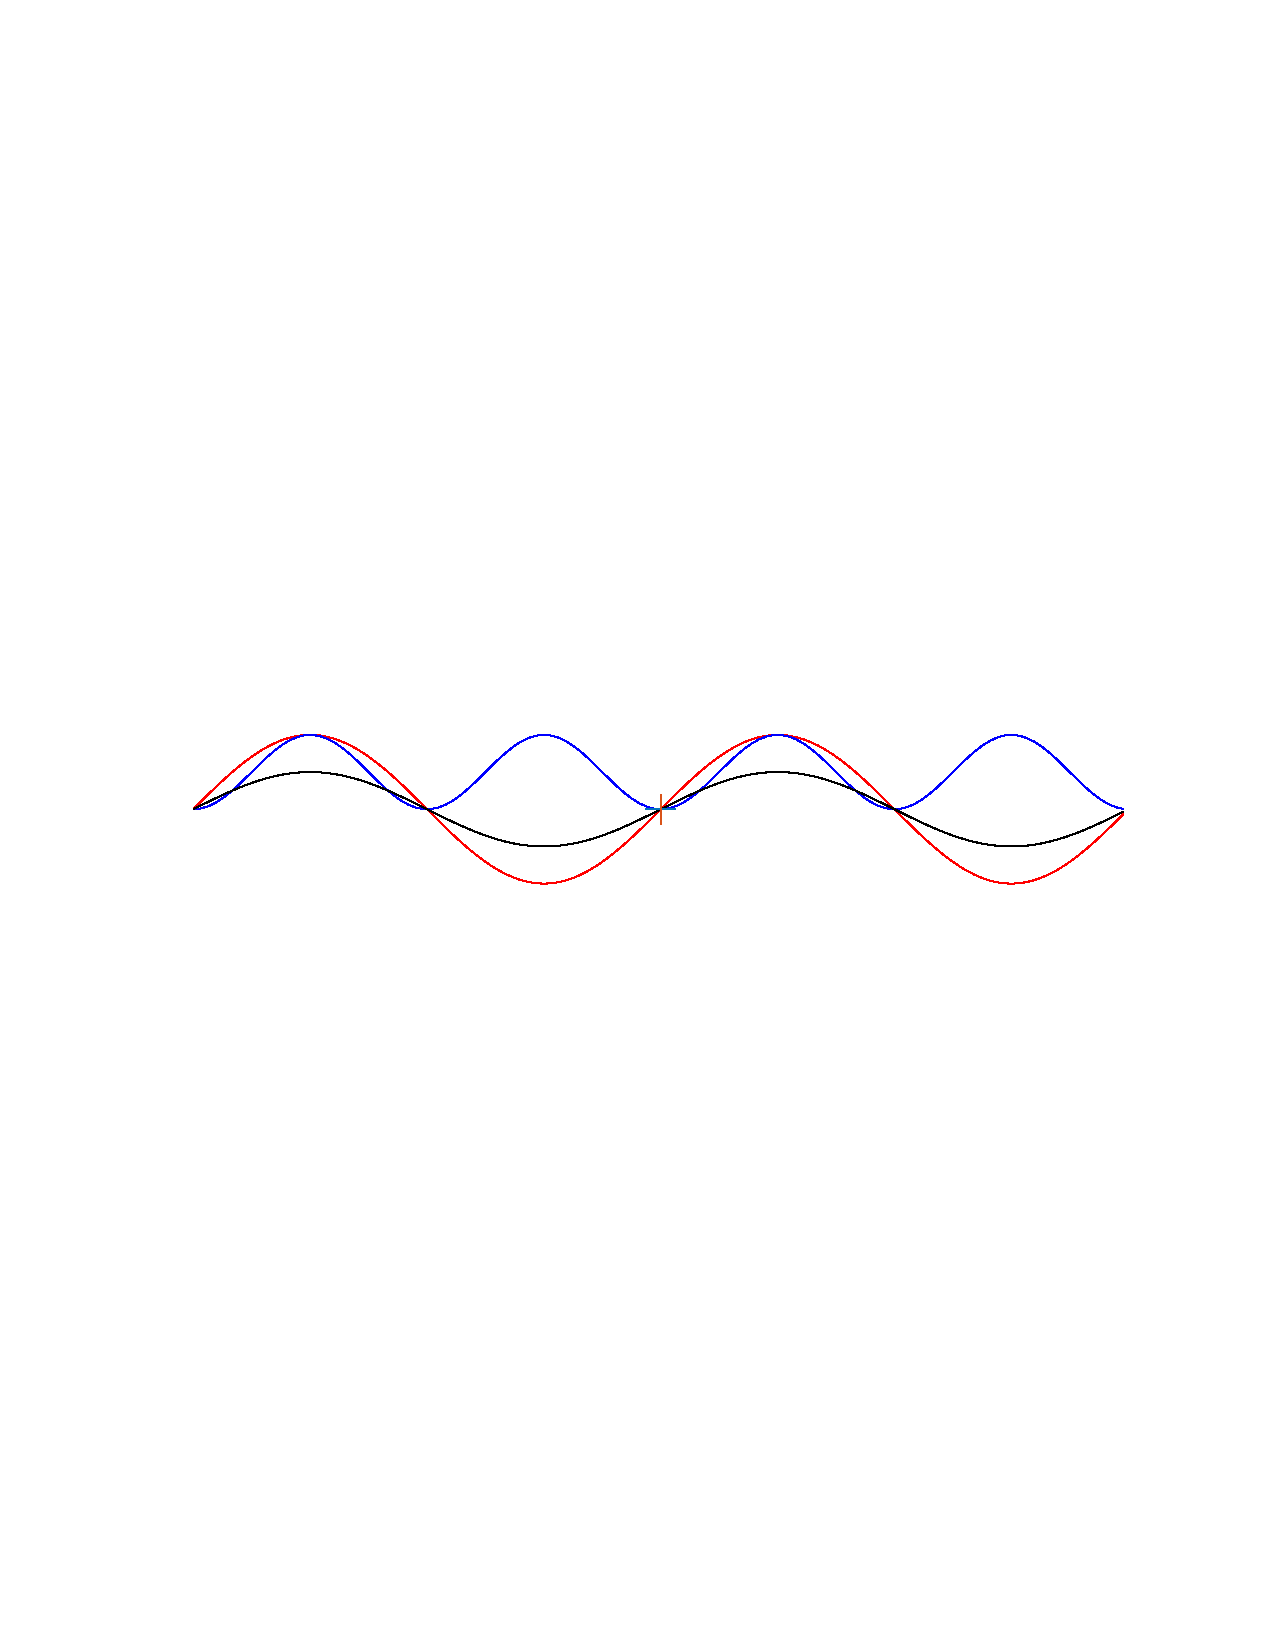
\includegraphics[scale=1,trim={70pt 320pt 70pt 320pt},clip]{myfigure}};
		
		\draw [-angle 60, thick] (-7.5,0.27) -- (9,0.27);
		\draw [-angle 60, thick] (0.39,-2) -- (0.39,3);
		
		\node at (6.7,-1.3) {$f(x) = \sin(x)$};
		\node at (6.7,1.8) {$g(x) = \sin^2(x)$};
		\node at (2.28,0.52) {$h(x) = \frac{\sin(x)}{2}$};
		\end{tikzpicture}
		\caption{Wykresy funkcji}
		\label{fig:funkcje}
	\end{figure}
\end{document}